\documentclass[twoside]{book}

% Packages required by doxygen
\usepackage{fixltx2e}
\usepackage{calc}
\usepackage{doxygen}
\usepackage[export]{adjustbox} % also loads graphicx
\usepackage{graphicx}
\usepackage[utf8]{inputenc}
\usepackage{makeidx}
\usepackage{multicol}
\usepackage{multirow}
\PassOptionsToPackage{warn}{textcomp}
\usepackage{textcomp}
\usepackage[nointegrals]{wasysym}
\usepackage[table]{xcolor}

% Font selection
\usepackage[T1]{fontenc}
\usepackage[scaled=.90]{helvet}
\usepackage{courier}
\usepackage{amssymb}
\usepackage{sectsty}
\renewcommand{\familydefault}{\sfdefault}
\allsectionsfont{%
  \fontseries{bc}\selectfont%
  \color{darkgray}%
}
\renewcommand{\DoxyLabelFont}{%
  \fontseries{bc}\selectfont%
  \color{darkgray}%
}
\newcommand{\+}{\discretionary{\mbox{\scriptsize$\hookleftarrow$}}{}{}}

% Page & text layout
\usepackage{geometry}
\geometry{%
  a4paper,%
  top=2.5cm,%
  bottom=2.5cm,%
  left=2.5cm,%
  right=2.5cm%
}
\tolerance=750
\hfuzz=15pt
\hbadness=750
\setlength{\emergencystretch}{15pt}
\setlength{\parindent}{0cm}
\setlength{\parskip}{3ex plus 2ex minus 2ex}
\makeatletter
\renewcommand{\paragraph}{%
  \@startsection{paragraph}{4}{0ex}{-1.0ex}{1.0ex}{%
    \normalfont\normalsize\bfseries\SS@parafont%
  }%
}
\renewcommand{\subparagraph}{%
  \@startsection{subparagraph}{5}{0ex}{-1.0ex}{1.0ex}{%
    \normalfont\normalsize\bfseries\SS@subparafont%
  }%
}
\makeatother

% Headers & footers
\usepackage{fancyhdr}
\pagestyle{fancyplain}
\fancyhead[LE]{\fancyplain{}{\bfseries\thepage}}
\fancyhead[CE]{\fancyplain{}{}}
\fancyhead[RE]{\fancyplain{}{\bfseries\leftmark}}
\fancyhead[LO]{\fancyplain{}{\bfseries\rightmark}}
\fancyhead[CO]{\fancyplain{}{}}
\fancyhead[RO]{\fancyplain{}{\bfseries\thepage}}
\fancyfoot[LE]{\fancyplain{}{}}
\fancyfoot[CE]{\fancyplain{}{}}
\fancyfoot[RE]{\fancyplain{}{\bfseries\scriptsize Generated by Doxygen }}
\fancyfoot[LO]{\fancyplain{}{\bfseries\scriptsize Generated by Doxygen }}
\fancyfoot[CO]{\fancyplain{}{}}
\fancyfoot[RO]{\fancyplain{}{}}
\renewcommand{\footrulewidth}{0.4pt}
\renewcommand{\chaptermark}[1]{%
  \markboth{#1}{}%
}
\renewcommand{\sectionmark}[1]{%
  \markright{\thesection\ #1}%
}

% Indices & bibliography
\usepackage{natbib}
\usepackage[titles]{tocloft}
\setcounter{tocdepth}{3}
\setcounter{secnumdepth}{5}
\makeindex

% Hyperlinks (required, but should be loaded last)
\usepackage{ifpdf}
\ifpdf
  \usepackage[pdftex,pagebackref=true]{hyperref}
\else
  \usepackage[ps2pdf,pagebackref=true]{hyperref}
\fi
\hypersetup{%
  colorlinks=true,%
  linkcolor=blue,%
  citecolor=blue,%
  unicode%
}

% Custom commands
\newcommand{\clearemptydoublepage}{%
  \newpage{\pagestyle{empty}\cleardoublepage}%
}

\usepackage{caption}
\captionsetup{labelsep=space,justification=centering,font={bf},singlelinecheck=off,skip=4pt,position=top}

%===== C O N T E N T S =====

\begin{document}

% Titlepage & ToC
\hypersetup{pageanchor=false,
             bookmarksnumbered=true,
             pdfencoding=unicode
            }
\pagenumbering{alph}
\begin{titlepage}
\vspace*{7cm}
\begin{center}%
{\Large enigme avec fichier \\[1ex]\large 1.\+0 }\\
\vspace*{1cm}
{\large Generated by Doxygen 1.8.13}\\
\end{center}
\end{titlepage}
\clearemptydoublepage
\pagenumbering{roman}
\tableofcontents
\clearemptydoublepage
\pagenumbering{arabic}
\hypersetup{pageanchor=true}

%--- Begin generated contents ---
\chapter{Data Structure Index}
\section{Data Structures}
Here are the data structures with brief descriptions\+:\begin{DoxyCompactList}
\item\contentsline{section}{\hyperlink{structenigme}{enigme} \\*Enigme struct }{\pageref{structenigme}}{}
\end{DoxyCompactList}

\chapter{File Index}
\section{File List}
Here is a list of all documented files with brief descriptions\+:\begin{DoxyCompactList}
\item\contentsline{section}{\hyperlink{enig_8c}{enig.\+c} }{\pageref{enig_8c}}{}
\item\contentsline{section}{\hyperlink{enig_8h}{enig.\+h} }{\pageref{enig_8h}}{}
\item\contentsline{section}{\hyperlink{main_8c}{main.\+c} \\*Main enigme }{\pageref{main_8c}}{}
\end{DoxyCompactList}

\chapter{Data Structure Documentation}
\hypertarget{structenigme}{}\section{enigme Struct Reference}
\label{structenigme}\index{enigme@{enigme}}


enigme struct  




{\ttfamily \#include $<$enig.\+h$>$}

\subsection*{Data Fields}
\begin{DoxyCompactItemize}
\item 
\mbox{\Hypertarget{structenigme_ac5c2141e5f8c366ff16d1fad83ee3e54}\label{structenigme_ac5c2141e5f8c366ff16d1fad83ee3e54}} 
S\+D\+L\+\_\+\+Surface $\ast$ {\bfseries img}
\item 
S\+D\+L\+\_\+\+Surface $\ast$ \hyperlink{structenigme_ad15bfe1f4b842b8694dd64dc29c65d8d}{lpoint}
\item 
\mbox{\Hypertarget{structenigme_a1ecc3fa572d2c308e1aecacf74fd1ec0}\label{structenigme_a1ecc3fa572d2c308e1aecacf74fd1ec0}} 
S\+D\+L\+\_\+\+Rect {\bfseries p}
\item 
S\+D\+L\+\_\+\+Rect \hyperlink{structenigme_a67e3facd55ae7707e4e339a1bbeee064}{lpointpos}
\end{DoxyCompactItemize}


\subsection{Detailed Description}
enigme struct 

\subsection{Field Documentation}
\mbox{\Hypertarget{structenigme_ad15bfe1f4b842b8694dd64dc29c65d8d}\label{structenigme_ad15bfe1f4b842b8694dd64dc29c65d8d}} 
\index{enigme@{enigme}!lpoint@{lpoint}}
\index{lpoint@{lpoint}!enigme@{enigme}}
\subsubsection{\texorpdfstring{lpoint}{lpoint}}
{\footnotesize\ttfamily S\+D\+L\+\_\+\+Surface $\ast$ enigme\+::lpoint}

Surface. \mbox{\Hypertarget{structenigme_a67e3facd55ae7707e4e339a1bbeee064}\label{structenigme_a67e3facd55ae7707e4e339a1bbeee064}} 
\index{enigme@{enigme}!lpointpos@{lpointpos}}
\index{lpointpos@{lpointpos}!enigme@{enigme}}
\subsubsection{\texorpdfstring{lpointpos}{lpointpos}}
{\footnotesize\ttfamily S\+D\+L\+\_\+\+Rect enigme\+::lpointpos}

Rectangle 

The documentation for this struct was generated from the following file\+:\begin{DoxyCompactItemize}
\item 
\hyperlink{enig_8h}{enig.\+h}\end{DoxyCompactItemize}

\chapter{File Documentation}
\hypertarget{enig_8c}{}\section{enig.\+c File Reference}
\label{enig_8c}\index{enig.\+c@{enig.\+c}}
{\ttfamily \#include $<$stdio.\+h$>$}\newline
{\ttfamily \#include $<$stdlib.\+h$>$}\newline
{\ttfamily \#include $<$string.\+h$>$}\newline
{\ttfamily \#include $<$S\+D\+L/\+S\+D\+L.\+h$>$}\newline
{\ttfamily \#include $<$S\+D\+L/\+S\+D\+L\+\_\+mixer.\+h$>$}\newline
{\ttfamily \#include $<$S\+D\+L/\+S\+D\+L\+\_\+image.\+h$>$}\newline
{\ttfamily \#include \char`\"{}enig.\+h\char`\"{}}\newline
Include dependency graph for enig.\+c\+:
\nopagebreak
\begin{figure}[H]
\begin{center}
\leavevmode
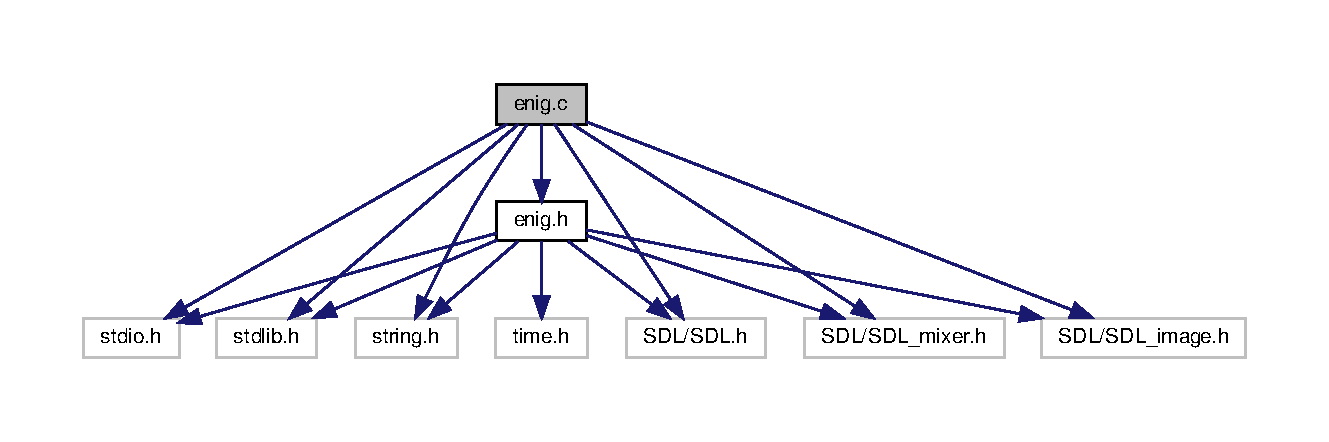
\includegraphics[width=350pt]{enig_8c__incl}
\end{center}
\end{figure}
\subsection*{Macros}
\begin{DoxyCompactItemize}
\item 
\mbox{\Hypertarget{enig_8c_a7a9a231e30b47bc0345749c8bd1e5077}\label{enig_8c_a7a9a231e30b47bc0345749c8bd1e5077}} 
\#define {\bfseries M\+A\+X\+\_\+\+L\+E\+N\+G\+TH}~100
\end{DoxyCompactItemize}
\subsection*{Functions}
\begin{DoxyCompactItemize}
\item 
void \hyperlink{enig_8c_a4d4ead3f0d4bf7d353da40004f7de4a4}{generate\+\_\+a} (S\+D\+L\+\_\+\+Surface $\ast$screen, char $\ast$chaine)
\begin{DoxyCompactList}\small\item\em To generate an enigme randomly. \end{DoxyCompactList}\item 
void \hyperlink{enig_8c_ae5f091f4e12f0ce070f3001464c9f5ca}{aff\+\_\+enigme} (\hyperlink{structenigme}{enigme} $\ast$e, S\+D\+L\+\_\+\+Surface $\ast$screen)
\begin{DoxyCompactList}\small\item\em To display the enigma. \end{DoxyCompactList}\item 
int \hyperlink{enig_8c_ae93c62d7e840b8843567985ba9ae9633}{solution\+\_\+e} (char $\ast$chaine)
\begin{DoxyCompactList}\small\item\em register the solution for each enigma \end{DoxyCompactList}\item 
int \hyperlink{enig_8c_ae855a03b9d7f7619bac3843306965df9}{resolution} (int $\ast$running, int $\ast$run)
\begin{DoxyCompactList}\small\item\em read the imput \end{DoxyCompactList}\item 
void \hyperlink{enig_8c_a4000acf4af9607e9d50a33b70643a99a}{afficher\+\_\+resultat} (S\+D\+L\+\_\+\+Surface $\ast$screen, int s, int r, \hyperlink{structenigme}{enigme} $\ast$en)
\begin{DoxyCompactList}\small\item\em To display the enigma result. \end{DoxyCompactList}\end{DoxyCompactItemize}


\subsection{Function Documentation}
\mbox{\Hypertarget{enig_8c_ae5f091f4e12f0ce070f3001464c9f5ca}\label{enig_8c_ae5f091f4e12f0ce070f3001464c9f5ca}} 
\index{enig.\+c@{enig.\+c}!aff\+\_\+enigme@{aff\+\_\+enigme}}
\index{aff\+\_\+enigme@{aff\+\_\+enigme}!enig.\+c@{enig.\+c}}
\subsubsection{\texorpdfstring{aff\+\_\+enigme()}{aff\_enigme()}}
{\footnotesize\ttfamily void aff\+\_\+enigme (\begin{DoxyParamCaption}\item[{\hyperlink{structenigme}{enigme} $\ast$}]{e,  }\item[{S\+D\+L\+\_\+\+Surface $\ast$}]{screen }\end{DoxyParamCaption})}



To display the enigma. 


\begin{DoxyParams}{Parameters}
{\em S\+D\+L\+\_\+\+Surface} & $\ast$screen, \\
\hline
{\em e} & for enigme \\
\hline
\end{DoxyParams}
\begin{DoxyReturn}{Returns}
Nothing 
\end{DoxyReturn}
Here is the call graph for this function\+:
\nopagebreak
\begin{figure}[H]
\begin{center}
\leavevmode
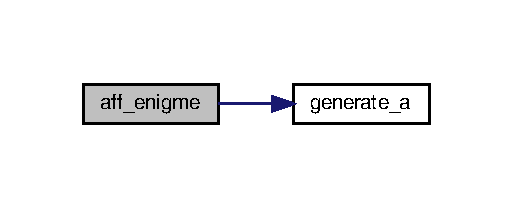
\includegraphics[width=246pt]{enig_8c_ae5f091f4e12f0ce070f3001464c9f5ca_cgraph}
\end{center}
\end{figure}
\mbox{\Hypertarget{enig_8c_a4000acf4af9607e9d50a33b70643a99a}\label{enig_8c_a4000acf4af9607e9d50a33b70643a99a}} 
\index{enig.\+c@{enig.\+c}!afficher\+\_\+resultat@{afficher\+\_\+resultat}}
\index{afficher\+\_\+resultat@{afficher\+\_\+resultat}!enig.\+c@{enig.\+c}}
\subsubsection{\texorpdfstring{afficher\+\_\+resultat()}{afficher\_resultat()}}
{\footnotesize\ttfamily void afficher\+\_\+resultat (\begin{DoxyParamCaption}\item[{S\+D\+L\+\_\+\+Surface $\ast$}]{screen,  }\item[{int}]{s,  }\item[{int}]{r,  }\item[{\hyperlink{structenigme}{enigme} $\ast$}]{en }\end{DoxyParamCaption})}



To display the enigma result. 


\begin{DoxyParams}{Parameters}
{\em S\+D\+L\+\_\+\+Surface} & $\ast$screen, en for enigme \\
\hline
{\em int} & s,r \\
\hline
\end{DoxyParams}
\begin{DoxyReturn}{Returns}
Nothing 
\end{DoxyReturn}
\mbox{\Hypertarget{enig_8c_a4d4ead3f0d4bf7d353da40004f7de4a4}\label{enig_8c_a4d4ead3f0d4bf7d353da40004f7de4a4}} 
\index{enig.\+c@{enig.\+c}!generate\+\_\+a@{generate\+\_\+a}}
\index{generate\+\_\+a@{generate\+\_\+a}!enig.\+c@{enig.\+c}}
\subsubsection{\texorpdfstring{generate\+\_\+a()}{generate\_a()}}
{\footnotesize\ttfamily void generate\+\_\+a (\begin{DoxyParamCaption}\item[{S\+D\+L\+\_\+\+Surface $\ast$}]{screen,  }\item[{char $\ast$}]{chaine }\end{DoxyParamCaption})}



To generate an enigme randomly. 


\begin{DoxyParams}{Parameters}
{\em S\+D\+L\+\_\+\+Surface} & $\ast$screen \\
\hline
{\em char} & $\ast$chaine \\
\hline
\end{DoxyParams}
\begin{DoxyReturn}{Returns}
Nothing 
\end{DoxyReturn}
Here is the caller graph for this function\+:
\nopagebreak
\begin{figure}[H]
\begin{center}
\leavevmode
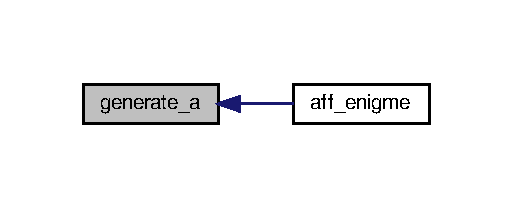
\includegraphics[width=246pt]{enig_8c_a4d4ead3f0d4bf7d353da40004f7de4a4_icgraph}
\end{center}
\end{figure}
\mbox{\Hypertarget{enig_8c_ae855a03b9d7f7619bac3843306965df9}\label{enig_8c_ae855a03b9d7f7619bac3843306965df9}} 
\index{enig.\+c@{enig.\+c}!resolution@{resolution}}
\index{resolution@{resolution}!enig.\+c@{enig.\+c}}
\subsubsection{\texorpdfstring{resolution()}{resolution()}}
{\footnotesize\ttfamily int resolution (\begin{DoxyParamCaption}\item[{int $\ast$}]{running,  }\item[{int $\ast$}]{run }\end{DoxyParamCaption})}



read the imput 


\begin{DoxyParams}{Parameters}
{\em int} & running, run \\
\hline
\end{DoxyParams}
\begin{DoxyReturn}{Returns}
r 
\end{DoxyReturn}
\mbox{\Hypertarget{enig_8c_ae93c62d7e840b8843567985ba9ae9633}\label{enig_8c_ae93c62d7e840b8843567985ba9ae9633}} 
\index{enig.\+c@{enig.\+c}!solution\+\_\+e@{solution\+\_\+e}}
\index{solution\+\_\+e@{solution\+\_\+e}!enig.\+c@{enig.\+c}}
\subsubsection{\texorpdfstring{solution\+\_\+e()}{solution\_e()}}
{\footnotesize\ttfamily int solution\+\_\+e (\begin{DoxyParamCaption}\item[{char $\ast$}]{chaine }\end{DoxyParamCaption})}



register the solution for each enigma 


\begin{DoxyParams}{Parameters}
{\em char} & $\ast$chaine \\
\hline
\end{DoxyParams}
\begin{DoxyReturn}{Returns}
solution 
\end{DoxyReturn}

\hypertarget{enig_8h}{}\section{enig.\+h File Reference}
\label{enig_8h}\index{enig.\+h@{enig.\+h}}
{\ttfamily \#include $<$S\+D\+L/\+S\+D\+L.\+h$>$}\newline
{\ttfamily \#include $<$S\+D\+L/\+S\+D\+L\+\_\+mixer.\+h$>$}\newline
{\ttfamily \#include $<$S\+D\+L/\+S\+D\+L\+\_\+image.\+h$>$}\newline
{\ttfamily \#include $<$time.\+h$>$}\newline
{\ttfamily \#include $<$stdio.\+h$>$}\newline
{\ttfamily \#include $<$stdlib.\+h$>$}\newline
{\ttfamily \#include $<$string.\+h$>$}\newline
Include dependency graph for enig.\+h\+:
\nopagebreak
\begin{figure}[H]
\begin{center}
\leavevmode
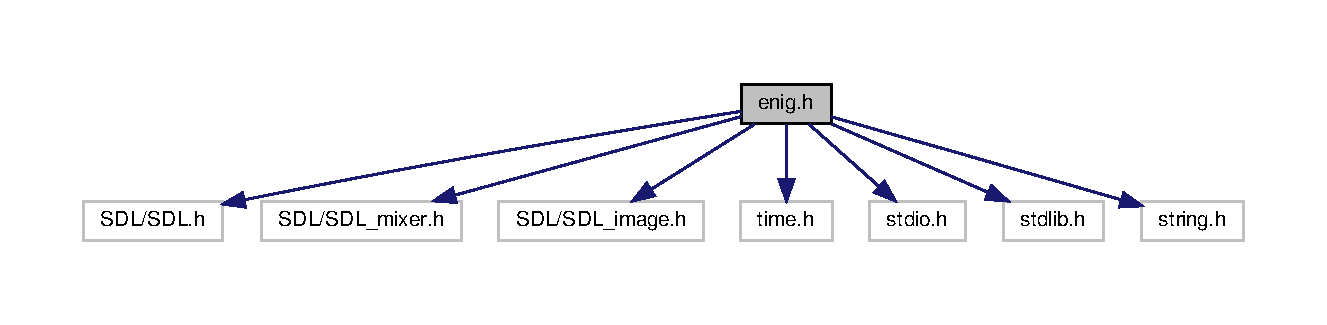
\includegraphics[width=350pt]{enig_8h__incl}
\end{center}
\end{figure}
This graph shows which files directly or indirectly include this file\+:
\nopagebreak
\begin{figure}[H]
\begin{center}
\leavevmode
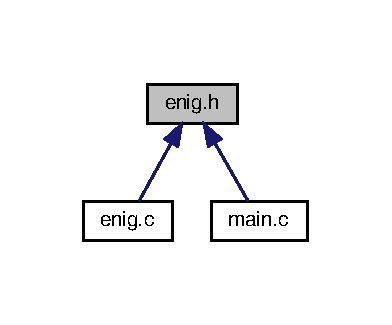
\includegraphics[width=188pt]{enig_8h__dep__incl}
\end{center}
\end{figure}
\subsection*{Data Structures}
\begin{DoxyCompactItemize}
\item 
struct \hyperlink{structenigme}{enigme}
\begin{DoxyCompactList}\small\item\em enigme struct \end{DoxyCompactList}\end{DoxyCompactItemize}
\subsection*{Functions}
\begin{DoxyCompactItemize}
\item 
\mbox{\Hypertarget{enig_8h_a94c8be36e6ac47cec69c5ff3881d9b7b}\label{enig_8h_a94c8be36e6ac47cec69c5ff3881d9b7b}} 
void {\bfseries aff\+\_\+enigme} (\hyperlink{structenigme}{enigme} $\ast$e, S\+D\+L\+\_\+\+Surface $\ast$screen, char image\mbox{[}$\,$\mbox{]}, char $\ast$chaine)
\item 
\mbox{\Hypertarget{enig_8h_a28a6f5121865882fecf2b01291e4b35f}\label{enig_8h_a28a6f5121865882fecf2b01291e4b35f}} 
void {\bfseries generate\+\_\+a} (S\+D\+L\+\_\+\+Surface $\ast$screen, char image \mbox{[}$\,$\mbox{]})
\item 
\mbox{\Hypertarget{enig_8h_a56e8098a699d9adc047b50e4315e9db4}\label{enig_8h_a56e8098a699d9adc047b50e4315e9db4}} 
int {\bfseries solution\+\_\+e} (char image \mbox{[}$\,$\mbox{]}, char $\ast$chaine)
\item 
int \hyperlink{enig_8h_ae855a03b9d7f7619bac3843306965df9}{resolution} (int $\ast$running, int $\ast$run)
\begin{DoxyCompactList}\small\item\em read the imput \end{DoxyCompactList}\item 
void \hyperlink{enig_8h_a4000acf4af9607e9d50a33b70643a99a}{afficher\+\_\+resultat} (S\+D\+L\+\_\+\+Surface $\ast$screen, int s, int r, \hyperlink{structenigme}{enigme} $\ast$en)
\begin{DoxyCompactList}\small\item\em To display the enigma result. \end{DoxyCompactList}\end{DoxyCompactItemize}


\subsection{Function Documentation}
\mbox{\Hypertarget{enig_8h_a4000acf4af9607e9d50a33b70643a99a}\label{enig_8h_a4000acf4af9607e9d50a33b70643a99a}} 
\index{enig.\+h@{enig.\+h}!afficher\+\_\+resultat@{afficher\+\_\+resultat}}
\index{afficher\+\_\+resultat@{afficher\+\_\+resultat}!enig.\+h@{enig.\+h}}
\subsubsection{\texorpdfstring{afficher\+\_\+resultat()}{afficher\_resultat()}}
{\footnotesize\ttfamily void afficher\+\_\+resultat (\begin{DoxyParamCaption}\item[{S\+D\+L\+\_\+\+Surface $\ast$}]{screen,  }\item[{int}]{s,  }\item[{int}]{r,  }\item[{\hyperlink{structenigme}{enigme} $\ast$}]{en }\end{DoxyParamCaption})}



To display the enigma result. 


\begin{DoxyParams}{Parameters}
{\em S\+D\+L\+\_\+\+Surface} & $\ast$screen, en for enigme \\
\hline
{\em int} & s,r \\
\hline
\end{DoxyParams}
\begin{DoxyReturn}{Returns}
Nothing 
\end{DoxyReturn}
\mbox{\Hypertarget{enig_8h_ae855a03b9d7f7619bac3843306965df9}\label{enig_8h_ae855a03b9d7f7619bac3843306965df9}} 
\index{enig.\+h@{enig.\+h}!resolution@{resolution}}
\index{resolution@{resolution}!enig.\+h@{enig.\+h}}
\subsubsection{\texorpdfstring{resolution()}{resolution()}}
{\footnotesize\ttfamily int resolution (\begin{DoxyParamCaption}\item[{int $\ast$}]{running,  }\item[{int $\ast$}]{run }\end{DoxyParamCaption})}



read the imput 


\begin{DoxyParams}{Parameters}
{\em int} & running, run \\
\hline
\end{DoxyParams}
\begin{DoxyReturn}{Returns}
r 
\end{DoxyReturn}

\hypertarget{main_8c}{}\section{main.\+c File Reference}
\label{main_8c}\index{main.\+c@{main.\+c}}


Main enigme.  


{\ttfamily \#include $<$stdio.\+h$>$}\newline
{\ttfamily \#include $<$stdlib.\+h$>$}\newline
{\ttfamily \#include $<$string.\+h$>$}\newline
{\ttfamily \#include $<$S\+D\+L/\+S\+D\+L.\+h$>$}\newline
{\ttfamily \#include $<$S\+D\+L/\+S\+D\+L\+\_\+image.\+h$>$}\newline
{\ttfamily \#include \char`\"{}enig.\+h\char`\"{}}\newline
{\ttfamily \#include $<$time.\+h$>$}\newline
Include dependency graph for main.\+c\+:
\nopagebreak
\begin{figure}[H]
\begin{center}
\leavevmode
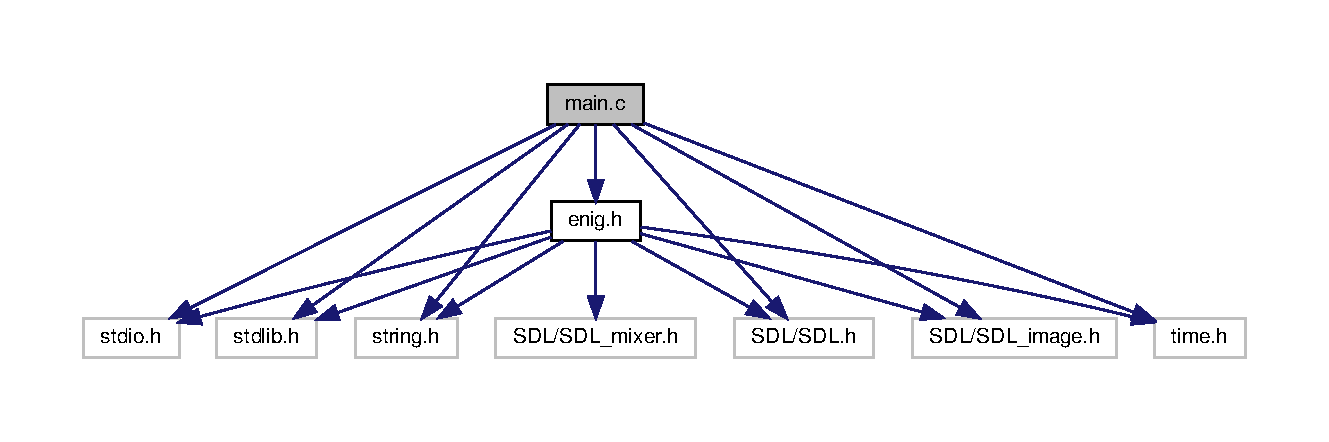
\includegraphics[width=350pt]{main_8c__incl}
\end{center}
\end{figure}
\subsection*{Macros}
\begin{DoxyCompactItemize}
\item 
\mbox{\Hypertarget{main_8c_a7a9a231e30b47bc0345749c8bd1e5077}\label{main_8c_a7a9a231e30b47bc0345749c8bd1e5077}} 
\#define {\bfseries M\+A\+X\+\_\+\+L\+E\+N\+G\+TH}~100
\end{DoxyCompactItemize}
\subsection*{Functions}
\begin{DoxyCompactItemize}
\item 
\mbox{\Hypertarget{main_8c_ae66f6b31b5ad750f1fe042a706a4e3d4}\label{main_8c_ae66f6b31b5ad750f1fe042a706a4e3d4}} 
int {\bfseries main} ()
\end{DoxyCompactItemize}


\subsection{Detailed Description}
Main enigme. 

\begin{DoxyAuthor}{Author}
Iskander 
\end{DoxyAuthor}
\begin{DoxyVersion}{Version}
1.\+0 
\end{DoxyVersion}
\begin{DoxyDate}{Date}
18/04/2021
\end{DoxyDate}
Making enigme for video game 
%--- End generated contents ---

% Index
\backmatter
\newpage
\phantomsection
\clearemptydoublepage
\addcontentsline{toc}{chapter}{Index}
\printindex

\end{document}
